%! Author = Charles Yang
%! Date = 8/24/2021

% Preamble
\documentclass[11pt]{article}

% Packages
\usepackage{amsmath}
\usepackage{amsfonts}
\usepackage{hyperref}
\usepackage{enumitem}
\usepackage{graphicx}

% Settings
\setlist[enumerate]{font=\bfseries}

% Title Info
\title{STAT 347 HW3}
\author{Charles Yang}

\addtolength{\oddsidemargin}{-.875in}
\addtolength{\evensidemargin}{-.875in}
\addtolength{\textwidth}{1.75in}
\addtolength{\topmargin}{-.875in}
\addtolength{\textheight}{1.75in}

% Document
\begin{document}
    \maketitle

    \begin{enumerate}

        \item[3.1]
        \begin{align*}
            P(0) &= 0.20 \\
            P(1) &= (0.4 - 0.1) + (0.5 - 0.1) = 0.70 \\
            P(2) &= 0.2 + 0.4 + 0.5 - 1 = 0.1
        \end{align*}

        \item[3.4]
        \begin{align*}
            P(0) &= P(v_1^c \cap (v_2^c \cup v_3^c)) = 0.2 * (0.2 + 0.2 - 0.04) = 0.072\\
            P(1) &= P(v_1 \cap (v_2^c \cup v_3^c)) + P(v_1^c \cap (v_2 \cap v_3)) \\
            &= 0.8 * (0.2 + 0.2 - 0.04) + 0.2 * (0.64) = 0.416 \\
            P(2) &= P(v_1 \cap v_2 \cap v_3) = 0.8^3 = 0.512
        \end{align*}

        \item[3.9]
        \begin{enumerate}
            \item[a]
            \begin{align*}
                P(0) &= C(3, 0)(0.95)^3(0.05)^0 = 0.8574 \\
                P(1) &= C(3, 1)(0.95)^2(0.05)^1 = 0.1354\\
                P(2) &= C(3, 2)(0.95)^1(0.05)^2 = 0.0071 \\
                P(3) &= C(3, 3)(0.95)^0(0.05)^3 = 0.0001
            \end{align*}
            \item[b]
            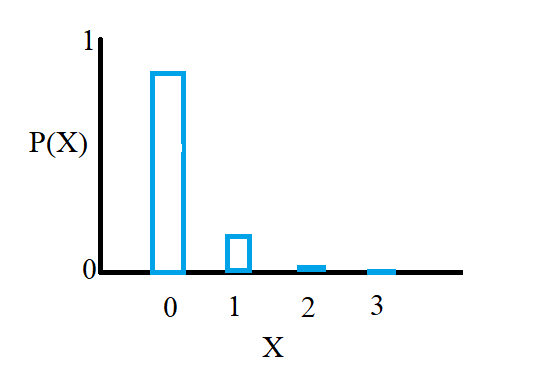
\includegraphics{3.9b.png}
            \newpage
            \item[c] $P(e > 1) = P(2) + P(3) = 0.0072$
        \end{enumerate}

        \item[3.12]
        \begin{align*}
            E(Y) &= 1*0.4 + 2*0.3 + 3*0.2 + 4*0.1 = 2.0 \\
            E(\frac{1}{Y}) &= \sum \frac{1}{Y}p(Y) \\
            &= \frac{1}{1}0.4 + \frac{1}{2}0.3 + \frac{1}{3}0.2 + \frac{1}{4}0.1 \\
            &= 0.642 \\
            E(Y^2 - 1) &= 1^2*0.4 + 2^2*0.3 + 3^2*0.2 + 4^2*0.1 - 1 \\
            &= 4 \text{ (Corollary:} E(Y^2) = 5) \\
            V(Y) &= E(Y^2) - E(Y)^2 \\
            &= 5 - 2^2 \\
            &= 1
        \end{align*}

        \item[3.14]
        \begin{enumerate}
            \item[a] $3*0.03 + 4*0.05 + 5*0.07 + 6*0.1 + 7*0.14 + 8*0.2 + 9*0.18 + 10*0.12 + 11*0.07 + 12*0.03 + 13*0.01 = 7.9$
            \item[b] $(3 - 7.9)^2*0.3 + (4 - 7.9)^2*0.05 + (5 - 7.9)^2*0.07 + (6 - 7.9)^2*0.1 + (7 - 7.9)^2*0.14 + (8 - 7.9)^2*0.2 + (9 - 7.9)^2*0.18 + (10 - 7.9)^2*0.12 + (11 - 7.9)^2*0.07 + (12 - 7.9)^2*0.03 + (13 - 7.9)^2*0.01$ \\
                    $= 3.349^2$
            \item[c] $\mu \pm 2\sigma = [4.551, 11.249]$, $P(5) + P(6) + P(7) + P(8) + P(9) + P(10) + P(11) = 0.88$
        \end{enumerate}

        \item[3.21] $E(8\pi R^2) = 8\pi (21^2*0.5+22^2*0.2+23^2*0.3+24^2*0.25+25*0.15+26^2*0.05) = 18788$

        \item[3.23] $P(15) = 8/52$, $P(5) = 8/52$, $P(4) = (52-16)/52$ \\
                    $15*(8/52) + 5*(8/52) + 4*(36/52) = 5.85$

        \item[3.30]
        \begin{enumerate}
            \item[a] The mean of x will be larger because all values of X are larger than their sibling values in Y
            \item[b] $E(X) = E(Y) + 1$. Yes
            \item[c] It should be the same. Shifting all values by 1 does not change the spread.
            \item[d]
            \begin{align*}
                V(X) &= E((X - E(X))^2) = \sigma^2 \\
                V(X) &= E((Y + 1 - E(Y + 1))^2) \\
                V(X) &= E((Y + 1 - (E(Y) + 1))^2) \\
                V(X) &= E((Y + 1 - E(Y) - 1)^2) \\
                V(X) &= E((Y - E(Y))^2) \\
                V(Y) &= E((Y - E(Y))^2) = \sigma^2
            \end{align*}
        \end{enumerate}
    \end{enumerate}
\end{document}